
\documentclass[review]{elsarticle}

\usepackage{lineno,hyperref}
\usepackage[mathletters]{ucs}
\usepackage[utf8x]{inputenc}
\usepackage[linesnumbered, ruled, vlined]{algorithm2e}
\usepackage{natbib}
\usepackage{supertabular}
\usepackage{fancybox}
\usepackage{acronym}
\usepackage{array}
\usepackage{booktabs}
\usepackage{graphicx}
\usepackage{rotating}
\usepackage{tabularx}
\usepackage{multirow}
\usepackage{hhline}
\usepackage{setspace}
\usepackage{placeins}
\usepackage{longtable}
\usepackage{listings}
\usepackage{epstopdf}
\usepackage{subfigure}
\usepackage{courier}
\usepackage{amsfonts}
\usepackage{morefloats}
\usepackage{lipsum}
\usepackage{mathtools}
\usepackage{amsthm,amsmath}

% table
\usepackage{makecell}
\usepackage{color, colortbl}
\definecolor{Gray}{gray}{0.9}

% appendix
\usepackage[titletoc,title]{appendix}
\usepackage{hyperref}
\usepackage{cleveref}

% norm


\modulolinenumbers[5]

\journal{Journal of Network and Computer Applications}

%%%%%%%%%%%%%%%%%%%%%%%
%% Elsevier bibliography styles
%%%%%%%%%%%%%%%%%%%%%%%
%% To change the style, put a % in front of the second line of the current style and
%% remove the % from the second line of the style you would like to use.
%%%%%%%%%%%%%%%%%%%%%%%

%% Numbered
%\bibliographystyle{model1-num-names}

%% Numbered without titles
%\bibliographystyle{model1a-num-names}

%% Harvard
%\bibliographystyle{model2-names.bst}\biboptions{authoryear}

%% Vancouver numbered
%\usepackage{numcompress}\bibliographystyle{model3-num-names}

%% Vancouver name/year
%\usepackage{numcompress}\bibliographystyle{model4-names}\biboptions{authoryear}

%% APA style
%\bibliographystyle{model5-names}\biboptions{authoryear}

%% AMA style
%\usepackage{numcompress}\bibliographystyle{model6-num-names}

%% `Elsevier LaTeX' style
\bibliographystyle{elsarticle-num}
%%%%%%%%%%%%%%%%%%%%%%%

\begin{document}

\begin{frontmatter}

\title{Moment Distances from Robust Subspace for Botnet Detection}

%% Group authors per affiliation:
\author[unbaddress]{Thiago P. B. Vieira}
\author[unbaddress]{Eduardo Said Calil Vilaça}
\author[unbaddress,Ilmenauaddress,Fraunhoferaddress]{João Paulo C. L. da Costa}
\author[unbaddress]{Rafael T. de Sousa Júnior}

\address[unbaddress]{Department of Electrical Engineering, University of Brasilia (UnB), 70910-900, Brasília-DF, Brazil}
\address[Ilmenauaddress]{Institute for Information Technology, Ilmenau University of Technology, Ilmenau, Germany}
\address[Fraunhoferaddress]{Fraunhofer Institute for Integrated Circuits IIS, Erlangen, Germany}


\begin{abstract}
Distributed attacks organized by botnet has increasing and demanding the development of counter measures in order to detect and avoid botnet's attacks. This paper proposes an approach based on higher moments distances from robust subspace for botnet detection, applied to new features generated by flow aggregation, in a semi-supervised fashion and without the computational cost of new robust subspace learning for new observations. Experimental results reveal that the proposed approach outperforms widely adopted algorithms and a method based on robust skewness for a public data set of botnet attacks.
\end{abstract}

\begin{keyword}
Network Anomaly Detection \sep Botnet Detection \sep Moments \sep Robust Principal Component Analysis \sep Mahalanobis Distance
\end{keyword}

\end{frontmatter}

\linenumbers

%%%%%%%%%%%%%%%%%%%%%%%%%%%%%%%%%%%%%%%%%%%%%%%%%%%%%%%%%%%%%%%%%%%%%%%%%%%%%%%%%%%%%%%%%%%%%%%%%%%%%%%%%%%%%%%%%%%%%%%%%%%%%%%%%%%%%%%%%%%%%%%%%%%%%%%%%%%%%%%%%%%%%%%%%%%%%%%%%%%%%%%%%%%%%%%%%%%%%%%%%%%%%%%%%%%%%%%%%%%%
\section{Introduction}
\label{sec:introduction}

Anomaly detection can be defined as the identification of rare and suspicions events by differing the normal or majority of the data. Anomalies are also referred to as outliers, novelties, noise or deviations, and can be related to network attacks, frauds or defects \cite{bhuyan2014network,ahmed2016survey}. Anomalies can be hard to identify and separate from normal data due to the rare occurrences of anomalies in comparison to normal events, therefore anomaly detection algorithms have to be high discriminative, robust to contamination and able to deal with the imbalanced data problem \cite{he2008learning}.

Several efforts and researches aim to avoid network attacks based on known attackers, fingerprints or other patterns. However, distributed attacks organized by botnet has increasing and demanding the development of counter measures in order to detect and avoid unknown attacks or even to deal with adversarial changes on behavior, location and other patterns, in order to avoid detection by behavioral or pattern based detection systems \cite{gu2008botminer, garcia2014empirical,khattak2015botflex,acarali2016survey,wang2017botnet,Wang2018ddosbotnetssurvey}. To face this problem, it is possible to adopt unsupervised or semi-supervised approaches for network anomaly detection, where it is not necessary known anomalies for training models \cite{moustafa2019holistic}.

Network anomaly detection problems are usually characterized by skewed and imbalanced data \cite{Phua2004minority,he2008learning,benson2010network}. Learning algorithms for imbalanced data has been a challenging research topic, considering that the fundamental issue with the imbalanced learning problem is the ability of imbalanced data to significantly compromise the performance of most standard learning algorithms \cite{he2008learning}. Some techniques can make the data discriminative for better results on the imbalanced learning problem: Data engineering (i.e. sampling \cite{he2008learning,gu2008botminer}, aggregation \cite{lakhina2005mining,gu2008botminer,callegari2011novel, garcia2014empirical, acarali2016survey}); Feature extraction (i.e. decomposition \cite{vaswani2018robust}, robust estimates \cite{zhou2017anomaly}). 

% He and Garcia \cite{he2008learning} present a classification of imbalanced learning methods as sampling, cost-sensitive learning, kernel-based, and active learning. For more information about learning methods from imbalanced data, we refer to He and Garcia \cite{he2008learning}.

% Say that the data is lognormal \cite{benson2010network} and link it to skewness https://www.weibull.com/hotwire/issue47/relbasics47.htm
Some widely adopted algorithms assume a gaussian distributed data, however this assumption may not be observed in real world problems, such as the case of network traffic analysis, where network traffic features are usually more characterized by skewed and heavy-tailed distributions \cite{lakhina2005mining,benson2010network}. Findings of Benson \emph{et al.}  \cite{benson2010network} indicate that certain positive skewed and heavy-tailed distributions can model data center switch traffic, and highlights a difference between the data center environment and the wide area network, where the long-tailed Pareto distribution typically shows the best fit \cite{benson2010network}. This findings show that the skeweness and heavy-tailed distributions can impact algorithms that rely on gaussian distributed data, as well as it can reveal characteristics that can be exploited in order to obtain accurate classifiers for network anomaly detection. Therefore, learning methods for imbalanced and skewed data have been attracted attention of researchers \cite{Phua2004minority,hubert2009robustskewed}. Skewness and kurtosis are higher moments that can have their measurement as very sensitive for outlier detection, considering that the properties of the kurtosis has been used to identify clusters or outliers \cite{pena2010eigenvectors}, while skewness has been used as adjust factor for outlier detection \cite{hubert2009robustskewed}.

Principal Component Analysis (PCA) is very sensitive to anomalies, thus outliers can corrupt the entire data or can be explored to highlight unexpected changes and indicate attacks or frauds \cite{callegari2011novel,Lee2013,vieira2017model}. However, PCA is not precise to reveal flows, time or detailed information for each anomaly, and sometimes relies into visual analysis for principal component selection. Robust Principal Component Analysis (RPCA) \cite{candes2011robust} is an extension of PCA that aims to be resilient to outliers by means of a robust subspace learning \cite{vaswani2018robust} for outlier corrupted data, decomposing a given data matrix $\textbf{X}$ into the sum of a low rank matrix $\textbf{L}$, whose column subspace gives the principal components, and a sparse matrix $\textbf{S}$, which refers to outliers’ matrix. Therefore, robust subspace learning has receiving a growing attention of researchers aiming the development of network anomaly detection systems \cite{rousseeuw1984mcd, rousseeuw1999fastmcd, hubert2005robpca,hubert2009robustskewed, pascoal2012robust, zhou2017anomaly}, considering outlier-robust methods and sparse-corruption methods \cite{lerman2018overview}.

Mahalanobis Distance (MD) is a generalized distance which is useful for determining the similarity between an unknown sample and a collection of known samples, by considering the correlations between the variables and their mean values. MD has been used for distance based anomaly detection with robust estimates in many areas, assuming that the Mahalanobis Distance between robust estimates and new observations can reveal anomalies.

We believe that the skewness of anomalous and normal traffic can highlight features for improving anomaly detection in imbalanced data. The botnet detection algorithms can also be improved by feature engineering from aggregated traffic, considering that new features can make the data more discriminative for imbalanced learning problems. We also believe that the distance between robust estimates of normal traffic and anomalies can highlight discrepancies and be used for botnet detection. Therefore, we propose an approach based on higher moments distances from robust subspace for botnet detection, applied to new features generated by flow aggregation. The proposed approach relies on a robust subspace of normal traffic for estimating higher moments. The anomaly detection for new observations evaluate the Mahalanobis distance between the robust higher moments and the higher moments of new observations, in a semi-supervised fashion and without the computational cost of new robust subspace learning for new observations.

We propose a sampling method based on data aggregation for discriminative feature engineering, considering that data aggregation is a widely adopted approach for feature engineering \cite{garcia2014empirical, chandrashekar2014survey,acarali2016survey} and network anomaly detection \cite{lakhina2005mining, callegari2011novel, vieira2017model}. We evaluate the accuracy of the proposed approach for botnet detection on the CTU-13 data set \cite{garcia2014empirical}, which is a large data set of normal, background and botnet traffic that has been adopted to deal with the lack of up-to-date real-world data sets for anomaly detection systems \cite{osanaiye2016distributed}.

Experimental evaluation compares our proposal to widely adopted algorithms for anomaly detection based on clustering and statistical approaches, which are K-means and Gaussian Mixture Model (GMM) \cite{gaddam2007kmeans,moustafa2019holistic}, respectively. We also evaluate the results of ROBPCA \cite{hubert2005robpca}, which is a method that also relies on robust estimates with adjusted outlyingness based on robust skewness.

The main contribution of this work is a novel semi-supervised method for botnet detection that obtain results with high rates of attack detection in an imbalanced and skewed data set.

This paper is organized as follows. In Section \ref{sec:review}, it is conducted a literature review of network anomaly detection, botnet detection, sampling and aggregation for imbalanced learning and robust based anomaly detection methods. Section \ref{sec:datamodel} presents the data model and the evaluated data set. Section \ref{sec:mdrs} describes the proposed approach for botnet detection. Section \ref{sec:experimentalresults} discusses the experimental validation and presents the results, and Section \ref{sec:conclusionandfutureworks} draws the conclusions and the suggestions for future work.

%%%%%%%%%%%%%%%%%%%%%%%%%%%%%%%%%%%%%%%%%%%%%%%%%%%%%%%%%%%%%%%%%%%%%%%%%%%%%%%%%%%%%%%%%%%%%%%%%%%%%%%%%%%%%%%%%%%%%%%%%%%%%%%%%%%%%%%%%%%%%%%%%%%%%%%%%%%%%%%%%%%%%%%%%%%%%%%%%%%%%%%%%%%%%%%%%%%%%%%%%%%%%%%%%%%%%%%%%%%%
% network anomaly detectiom, botnet detection, botnet detection approaches, approaches based on subspace learning, feature generation and aggregation, about the methodos to compare and metrics
\section{Literature Review}
\label{sec:review}

% network anomaly detectiom
Bhuyan \emph{et al.} \cite{bhuyan2014network} provide an overview of facets of network anomaly detection, present attacks normally encountered by network intrusion detection systems, and categorize existing network anomaly detection methods and systems based on the underlying techniques. Ahmed \emph{et al.} \cite{ahmed2016survey} present an analysis of four major categories of anomaly detection techniques which include classification, statistical, information theory and clustering. Moustafa \emph{et al.} \cite{moustafa2019holistic} discuss aspects of anomaly-based Network Intrusion Detection Systems (NIDSs), explains cyber-attacks and new solutions for anomaly detection, and provides a benchmark data sets for training and validating approaches for detection. 

% botnet detection
A botnet is a network of bots, that are compromised machines under the influence of malware (bot). The botnet is commandeered by a botmaster and used as resource for attacks, such as distributed denial-of-service (DDoS) attacks, and fraudulent activities such as spam, phishing, identity theft, and information ex-filtration. We refer to \cite{ahmed2016survey} and \cite{moustafa2019holistic} for an overview of network attacks. The botmaster coordinate a botnet through a command and control (C\&C) channel where bots receive commands and synchronize attacks and fraudulent activities. Centralized C\&C structures using the Internet Relay Chat (IRC) protocol have been utilized by botmasters for a long time, but other protocols, such as HTTP, and architectures, such as Peer-To-Peer, have also been adopted \cite{gu2008botminer}.

Acarali \emph{et al.} \cite{acarali2016survey} surveys network-based detection approaches for HTTP-based botnets, surveys traffic-based features used to detect bot traffic and presents an abstraction of the main types of features related to protocols and OSI layers. Wang \emph{et al.} \cite{Wang2018ddosbotnetssurvey} present an analysis based on 50,704 different Internet DDoS attacks originated of 674 botnets from 23 different botnet families with a total of 9,026 victim belonging to 1,074 organizations in 186 countries. Their analysis reveals that geolocation of the attacking sources follows patterns and enables source prediction, and highlights that multiple attacks to the same target also exhibit strong patterns of inter-attack time interval, also presents that there is a trend for different botnets to launch DDoS attacks targeting the same victim, simultaneously or in turn.

The BotHunter was proposed by Gu \emph{et al.} \cite{gu2007bothunter} to detect the infection and coordination of botnets by matching sequence model, through a correlation approach for detecting stages of the infection process.  Gu \emph{et al.} \cite{gu2008botminer} presented the BotMiner, which aims to detect groups of compromised machines that are part of a botnet. BotMiner monitors communications that may suggest C\&C or malicious activities, and finds a coordinated group pattern by means of clusters of similar communication activities, clusters of similar malicious activities, and performs cross cluster correlation to identify the hosts that share both similar communication patterns and similar malicious activity patterns.

Khattak \emph{et al.} \cite{khattak2015botflex} proposed BotFlex, which is a network-based tool for botnet detection, composed by a Complex Event Processing (CEP) engine and on a correlation framework that continuously receives events and correlates them according to rules. BotFlex's results are compared to BotHunter \cite{gu2007bothunter}, but the evaluation relies in a own and not public data set.

% justification for the data set and present who else use it
Several approaches for network attack detection uses the KDD 99 \cite{ahmed2016survey,osanaiye2016distributed,bhuyan2014network} data sets for accuracy and performance evaluation, due to their availability and labeled attacks. Even though the KDD 99 data set are criticized by the generation procedure and the risk of over-estimations of anomaly detection due to data redundancy, it still represents one of the few publicly available labeled data sets currently in use today by researchers \cite{osanaiye2016distributed,bhuyan2014network}. NSL-KDD \cite{tavallaee2009detailed} data set is the refined version of the KDD 99 data set that redundant data records are removed, in order to avoid biased classifications. However, NSL-KDD data set maintain the limitations of the KDD 99 regarding volume and reproduction of network traffic similar to the real networks.

The objective of Garcia \emph{et al.} \cite{garcia2014empirical} is to compare three botnet detection methods using a simple and reproducible methodology, and a good data set and a new error metric. This paper evaluates some data sets for network anomaly detection, surveys some approaches for botnet detection, proposes two methods (BClus and CAMNEP) for botnet detection and compare results to BotHunter \cite{gu2007bothunter}. Considering the lack of available labeled data sets, Garcia \emph{et al.} \cite{garcia2014empirical} proposes the CTU-13 data set, which is composed by attack, normal and background labeled data, in an imbalanced distribution like in a real network. The authors recommend that none of the botnet families used in the training and cross-validation data set should be used in the testing data set, aiming to ensure that the evaluated methods can generalize and detect new behaviors. Adopting the training and testing approach proposed by Garcia \emph{et al.}, some botnet malwares wouldn't be tested, since in the author's proposal some botnets are present only for training. 

Wang and Paschalidis \cite{wang2017botnet} proposed a botnet detection approach based on anomaly and community detection, aiming for detecting botnets and identifying bots before the botnet becomes active. The first stage detects anomalies by leveraging large deviations of an empirical distribution. The second stage detects the bots using ideas from social network community detection in a graph that captures correlations of interactions among nodes over time. This work is compared with the BotHunter \cite{gu2007bothunter} on the CTU-13 botnet data set \cite{garcia2014empirical}.

% \cite{da2018online} proposes an approach using the Very Fast Decision Tree, a classification algorithm used on stream mining that can learn incrementally when needed, to identify botnets by observing network flows. When evaluating the approach on multiple scenarios with different botnets, we were able to achieve high performance metrics on the majority of scenarios, while using a significantly low number of labelled instances. It discard scenarios 5 and 6. They does not compute F1, but it is easy to compute it from precision and recall provided.

% Anomaly detection by subspace larning
Traditional PCA-based anomaly detection models are not suitable for anomaly interpretation, as they judge whether a data instance is an anomaly or not based on the length of its projection on the abnormal subspace spanned by the less significant principal components, and there is no direct mapping between PCA’s dimensionality-reduced subspace and the original feature space \cite{ringberg2007sensitivity}. However, to overcome the above mentioned limitations, some approaches based on PCA have been proposed for network anomaly detection. Callegari \emph{et al.} \cite{callegari2011novel} proposed a PCA-based method for identifying the network traffic flows responsible for an anomaly detected at the aggregate level, by means of a separation of normal and anomalies according to principal components (normal) and remaining (anomalies). Lee \emph{et al.} \cite{Lee2013} presented OverSampling PCA (osPCA), which allows one to determine the anomaly of the target instance according to the variation of the resulting dominant eigenvector obtained by similarity analysis and over sampling. Vieira \emph{et al.} \cite{vieira2017model} proposed a framework that applies Model Order Selection (MOS) for detection of time frames under attack and uses similarity analysis to extract details and detect the time and ports under attack.

% Anomaly detection by robust subspace learning
The problem of PCA or subspace learning for outlier corrupted data is called robust PCA (RPCA) or robust subspace learning \cite{vaswani2018robust}, which can be defined as the decomposition of a given data matrix $\textbf{X}$ into the sum of a low rank matrix $\textbf{L}$, whose column subspace gives the principal components, and a sparse matrix $\textbf{S}$, with outliers or noise. This definition is also referred to as the sparse + low rank (S + LR) formulation \cite{vaswani2018robust}. We refer to \cite{lerman2018overview} and \cite{vaswani2018robust} for more details regarding robust subspace learning. 

Robust subspace learning has receiving a growing attention of researchers aiming the development of anomaly detection systems \cite{rousseeuw1984mcd, rousseeuw1999fastmcd}, considering outlier-robust methods and sparse-corruption methods \cite{lerman2018overview}. RPCA is been mainly applied to computer vision, in problems of robust subspace tracking and robust subspace recovery. However, RPCA has also been adopted for general outlier detection \cite{hubert2005robpca,hubert2009robustskewed,cherapanamjeri2017thresholding,zhou2017anomaly,NetflixSurus} and for anomaly detection on network traffic \cite{pascoal2012robust}. ROBPCA \cite{hubert2005robpca} intends to identify outliers using PCA from robust estimates of mean and covariance matrix, to reduce the data dimensions and plotting the orthogonal distances versus the robust score distances, to flag an outlier map. However, ROBPCA flags many points as outlying when the original data is skewed. Therefore, Hubert \emph{et al.} \cite{hubert2009robustskewed} proposed ROBPCA-AO, which improves ROBPCA for problems with skewed data, by means of an adjusted outlyingness based on robust skewness. 

Pascoal \emph{et al.} \cite{pascoal2012robust} proposed an approach based on a robust mutual information estimator for feature selection and based on RPCA for outlier detection in internet traffic. The anomaly detection proposed by Pascoal \emph{et al.} is an unsupervised approach that estimate the first $k$ robust principal components, calculate the score and the orthogonal distances, calculate the thresholds and classify new observations accordingly. 	Zhou and Paffenroth \cite{zhou2017anomaly} proposed the Robust Deep Autoencoders (RDA), which the central idea is that a RDA inherits the non-linear representation capabilities of autoencoders combined with the anomaly detection capabilities of RPCA. Considering that outliers and noise may reduce the quality of representations discovered by deep autoencoders, the proposed model isolates noise and outliers in the input by means of a RPCA approach, and the autoencoder is trained after this isolation. RDA was evaluated by the authors for the MNIST data set.

% feature engineering and aggregation
Lakhina \emph{et al.} \cite{lakhina2005mining} argue that the distributions of packet features (IP addresses and ports) observed in flow traces reveals both the presence and the structure of a wide range of anomalies. Lakhina \emph{et al.} show that the analysis of feature distributions leads to significant advances on sensitive detection of a wide range of anomalies, augmenting detection by volume-based methods, while the anomaly detection approach leads gains on automatic classification of anomalies via unsupervised learning. Goldberg and Shan \cite{goldberg2015importance} argue, based on experience and on published real-life examples of anomaly detectors in use at eBay, that processing monitored signals into features is a more fruitful for anomaly detection systems than devising complex statistical tests.

Benson \emph{et al.} \cite{benson2010network} conducted an empirical study of the network traffic in 10 data centers belonging to three different types of organizations, including university, enterprise, and cloud data centers. Findings of Benson \emph{et al.} indicate that certain positive skewed and heavy-tailed distributions can model data center switch traffic, and highlights a difference between the data center environment and the wide area network, where the long-tailed Pareto distribution typically shows the best fit \cite{benson2010network}. This findings highlight that the skeweness and heavy-tailed distributions can impact algorithms that rely on gaussian distributed data, as well as it can reveal characteristics that can be exploited in order to obtain accurate classifiers for network traffic analysis. 

Considering that learning methods for imbalanced and skewed data have been attracted attention of researchers \cite{Phua2004minority,hubert2009robustskewed}, higher moments can be used for outlier detection and discriminative analysis of skewed data. The skewness and kurtosis are higher moments that can contribute to sensitive outlier detectors, taking into account that the properties of the kurtosis can be used to identify clusters or outliers \cite{pena2010eigenvectors}, while skewness has been used as adjust factor for outlier detection in skewed data sets \cite{hubert2009robustskewed}.

We propose an approach based on higher moments distances from robust subspace for botnet detection, applied to new features generated by flow aggregation from the CTU-13 data set. The proposed approach relies on a robust subspace of normal traffic for estimating higher moments. Thus, we propose that the anomaly detection for new observations should evaluate the Mahalanobis distance between the robust higher moments and the higher moments of new observations, in a semi-supervised fashion and without the computational cost of new robust subspace learning for new observations. 

We propose a sampling method based on data aggregation for discriminative feature engineering, considering that data aggregation is a widely adopted approach for feature engineering \cite{garcia2014empirical, chandrashekar2014survey,acarali2016survey} and network anomaly detection \cite{lakhina2005mining, callegari2011novel, vieira2017model}. Finally, We evaluate the accuracy of the proposed approach for botnet detection on the CTU-13 data set \cite{garcia2014empirical}, which is a large data set of normal, background and botnet traffic that has been adopted to deal with the lack of up-to-date real-world data sets for anomaly detection systems \cite{osanaiye2016distributed}. 

%%%%%%%%%%%%%%%%%%%%%%%%%%%%%%%%%%%%%%%%%%%%%%%%%%%%%%%%%%%%%%%%%%%%%%%%%%%%%%%%%%%%%%%%%%%%%%%%%%%%%%%%%%%%%%%%%%%%%%%%%%%%%%%%%%%%%%%%%%%%%%%%%%%%%%%%%%%%%%%%%%%%%%%%%%%%%%%%%%%%%%%%%%%%%%%%%%%%%%%%%%%%%%%%%%%%%%%%%%%%
\section{Data Model}
\label{sec:datamodel}

In this paper, scalars are denoted by italic letters (\emph{a, b, A, B, $α$, $β$}), vectors by lowercase bold letters (\textbf{a, b}), matrices by uppercase bold letters (\textbf{A, B}), and $a_i,_j$ denotes the (\emph{i, j}) elements of the matrix \textbf{A}. The superscripts \textsuperscript{T} and \textsuperscript{-1} are used for matrix transposition and matrix inversion, respectively. The Frobenius norm is denoted as $\left\| \mathord{\cdot} \right\|_F$, while $\left\| \mathord{\cdot} \right\|_*$ denotes the nuclear norm of a matrix and $\left\| \mathord{\cdot} \right\|_1$ means the sum of the absolute values of matrix entries.

This section also presents a description of the data model in Subsection \ref{sec:CTU-13} and in Subsection \ref{sec:feat_eng} we describe the data aggregation and feature engineering adopted for the CTU-13.

\subsection{The CTU-13 data set}
\label{sec:CTU-13}

The CTU-13 is a data set of botnet traffic that was captured in the Czech Technical University \cite{garcia2014empirical}, by means of a testbed and execution of malwares in a real network. The CTU-13 data set contains 13 scenarios with network traffic of botnet malwares, that are: neris, rbot, virut, menti, sogou, nsys.ay and murlo. The types of C\&C and attack traffic present in CTU-13 data set are:

\begin{itemize}
	\item \textbf{Attacks:} Click Fraud (CF), Port Scan (PS), Compiled and Controlled by Authors (US), SPAM and DDOS;
	\item \textbf{C\&C:} IRC, P2P and HTTP.
\end{itemize}

We refer to Garcia \cite{garcia2014identifying} and Garcia \emph{et al.} \cite{garcia2014empirical} for a detailed description of the performed attacks and C\&C flows, also including the topology of the adopted testbed, rules for classifing normal flows, and an analysis of behaviors or patterns of the malware's traffic.

For all the scenarios, the authors of the CTU-13 data set convert the captured pcap files to NetFlows and release the processed flows. The data set contains ground-truth labels for flows as follows: flows from or to the infected machines are labeled as “botnet”; flows from or to well known and controlled machines are labeled as “normal”; all other flows are labeled as “background.”

The data set originally contains the following features by flows:  Start Time, End Time, Duration, Source IP Address, Source Port, Direction, Destination IP Address, Destination Port, State, Type of service from source to destination, Type of service from destination to source, Total of Packets and Total of Bytes.

Table \ref{tab:tab01} presents an overview organized by scenario and shows the malwares used for botnet attacks, the types of attacks and C\&C types, the total number of flows, the number of malicious flows, which includes flows of C\&C and attacks, and finally shows the number of normal flows.

\begin{table}[h!]
	\tiny
	\caption{CTU-13 data set Description}
	\label{tab:tab01}
	\begin{tabular}{| l | l | l | r | r | r | r | r | r | r | r | }
		\hline \rowcolor{Gray} \begin{tabular}[x]{@{}l@{}}\textbf{ID}\end{tabular}	&\begin{tabular}[x]{@{}l@{}}\textbf{Bot}\end{tabular}	 &\begin{tabular}[x]{@{}l@{}}\textbf{Type}\end{tabular}	&\begin{tabular}[x]{@{}l@{}}\textbf{Total}\end{tabular} &\begin{tabular}[x]{@{}l@{}}\textbf{Malicious}\end{tabular} &\begin{tabular}[x]{@{}l@{}}\textbf{C\&C}\end{tabular} &\begin{tabular}[x]{@{}l@{}}\textbf{Attack}\end{tabular} &\begin{tabular}[x]{@{}l@{}}\textbf{Normal}\end{tabular}\\ \hline
			10 & neris &\makecell[l]{IRC, Spam,\\CF} & 2,824,636 & 40,961 (1.45\%) & 341 (0.01\%) & 40,620 (1.44\%) &30,387 (1.07\%)\\ \hline
			11 & neris &\makecell[l]{IRC, Spam,\\CF} & 1,808,122 & 20,941 (1.16\%) & 673 (0.04\%) & 20,268 (1.12\%) &9,120 (0.5\%)\\ \hline
			12 & rbot &\makecell[l]{IRC, PS,\\US} & 4,710,638 & 26,822 (0.57\%) & 63 (0.00\%) & 26,759 (0.57\%) &116,887 (2.48\%)\\ \hline
			15 & rbot &\makecell[l]{IRC, DDoS,\\US} & 1,121,076 & 2,580 (0.23\%) & 52 (0.00\%) & 2,528 (0.23\%) &25,268 (2.25\%)\\ \hline
			15-2 & virut &\makecell[l]{Spam, PS,\\HTTP} & 129,832 & 901 (0.69\%) & 24 (0.02\%) & 877 (0.68\%) &4,679 (3.6\%)\\ \hline
			16 & menti &PS & 558,919 & 4,630 (0.83\%) & 199 (0.04\%) & 4,431 (0.79\%) &7,494 (1.34\%)\\ \hline
			16-2 & sogou &HTTP & 114,077 & 63 (0.06\%) & 26 (0.02\%) & 37 (0.03\%) &1,677 (1.47\%)\\ \hline
			16-3 & murlo &PS & 2,954,230 & 6,127 (0.21\%) & 1,074 (0.04\%) & 5,053 (0.17\%) &72,822 (2.46\%)\\ \hline
			17 & neris &\makecell[l]{IRC, Spam,\\CF, PS} & 2,087,508 & 184,987 (8.86\%) & 2,973 (0.14\%) & 182,014 (8.72\%) &43,340 (1.57\%)\\ \hline
			18 & rbot &\makecell[l]{IRC, DDoS,\\US} & 1,309,791 & 106,352 (8.12\%) & 33 (0.00\%) & 106,319 (8.12\%) &15,847 (1.2\%)\\ \hline
			18-2 & rbot &\makecell[l]{IRC, DDoS,\\US} & 107,251 & 8,164 (7.61\%) & 2 (0.00\%) & 8,162 (7.61\%) &2,718 (2.53\%)\\ \hline
			19 & nsys.ay &P2P & 325,471 & 2,168 (0.67\%) & 25 (0.01\%) & 2,143 (0.66\%) &7,628 (2.35\%)\\ \hline
			15-3 & virut &\makecell[l]{Spam, PS,\\HTTP} & 1,925,149 & 40,003 (2.08\%) & 536 (0.03\%) & 39,467 (2.05\%) &31,939 (1.65)\\ \hline
	\end{tabular}
\end{table}

The CTU-13 aims to reproduce the percentage of C\&C and attack flows according to real cases, where the number of malicious flows are very low in comparison to normal and background flows, resulting into a very imbalanced and challenging data set for botnet detection. 

An Exploratory Data Analysis (EDA) reveals that distributions of original features of the CTU-13 are skewed and present an overlapping between normal and anomalous flows. Following we present the Figure \ref{fig:fig01}, that presents the distribution of flow duration for scenario 12, and exemplifies the data skewness and overlapping. 

\begin{figure}[h!]
     \centering
     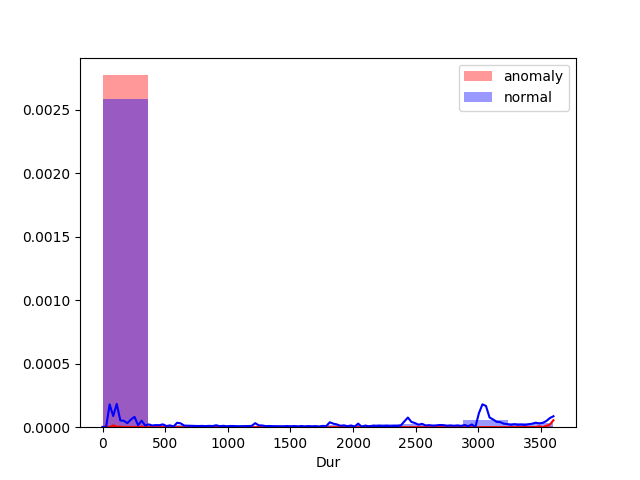
\includegraphics[width=8cm]{figures/raw_distplot_capture20110812_Dur.png}
     \caption{Distribution of flow duration for scenario 12.}
     \label{fig:fig01}
\end{figure}

To face data imbalance and skewness, we adopt a feature engineering by means of a sampling method based on data aggregation for obtaining more discriminative features, in accordance to important approaches for network anomaly detection \cite{lakhina2005mining, callegari2011novel, garcia2014empirical, chandrashekar2014survey,acarali2016survey, vieira2017model}.

\subsection{feature engineering}
\label{sec:feat_eng}

Related works proposed some features for improving network attack detection in various scenarios and approaches\cite{lakhina2005mining,gu2008botminer,callegari2011novel,chandrashekar2014survey,garcia2014empirical,acarali2016survey}. Inpired by these proposals and based on previous experience \cite{vieira2017model, galibus2017offline} and cross validation, we propose the following features for improving the anomaly detection by means of a method based on higher moments distances from robust subspace.
	
\begin{itemize}
	\item \textbf{total-flow-count :} Count of all flows.
	\item \textbf{known-flow-count:} Count of known flows, from controlled assets of the network, such routers, proxies, switches or machines that are part of the monitoring \cite{garcia2014identifying}.
	\item \textbf{avg-duration:} Average time of flows.
	\item \textbf{n-dports$<$1024:} Count of destinations ports lower than 1024.
	\item \textbf{n-sports$<$1024:} Count of source ports lower than 1024.
	\item \textbf{n-s-a-p-address:} Count of class A source address.
	\item \textbf{n-s-b-p-address:} Count of class B source address.
	\item \textbf{n-s-c-p-address:} Count of class C source address.
	\item \textbf{n-s-na-p-address:} Count of source address that are not class A, B or C, such as reserved class D and E addresses, IPV6 or internal address.
\end{itemize}

The proposed features are counting and average calculations, therefore it is necessary to adopt time windows to aggragate flows and calculate the features. We evaluate windows of 0.15 and 0.25 seconds, considering account that lower windows reduce the meantime between the data collection and results of the botnet detection approach, as well as permit to have more details to exactly identify malicious flows and attackers.

Figure \ref{fig:fig02} shows the distribution of average flow duration, for scenario 12, aggregated by windows of 0.15 seconds. In comparison to Figure \ref{fig:fig01}, that shows the distribution of flow duration for the same scenario, we can see that the feature based on aggration and on average flow duration is more discriminative and shows a better separation between normal and anomalous classes. Therefore, such data can improve the anomaly detection by learning algorithms.

\begin{figure}[h!]
     \centering
     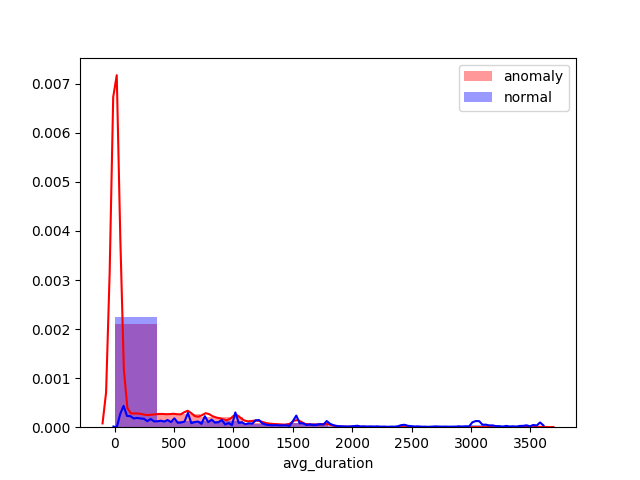
\includegraphics[width=8cm]{figures/agg_distplot_0_15s_12_avg_duration.png}
     \caption{Average flow duration for scenario 12, aggregated by 0.15 seconds.}
     \label{fig:fig02}
\end{figure}

The resulting data set is modeled into the matrix $\boldsymbol{X} \in \mathbb{R}^{n \times p}$ with $n$ rows as observations and $p$ columns of features, and is divided into scenarios, where each $i$-th scenario, presented by ID column in Table \ref{tab:tab01}, are represented as $\boldsymbol{X}_i$ and can be denoted as $\boldsymbol{X}_{18-2}$, for example. The normal traffic, required for trainning the semi-supervised approach, is denoted as $\boldsymbol{X}_i^r$

%%%%%%%%%%%%%%%%%%%%%%%%%%%%%%%%%%%%%%%%%%%%%%%%%%%%%%%%%%%%%%%%%%%%%%%%%%%%%%%%%%%%%%%%%%%%%%%%%%%%%%%%%%%%%%%%%%%%%%%%%%%%%%%%%%%%%%%%%%%%%%%%%%%%%%%%%%%%%%%%%%%%%%%%%%%%%%%%%%%%%%%%%%%%%%%%%%%%%%%%%%%%%%%%%%%%%%%%%%%%
\section{Moment Distances from Robust Subspace for Botnet Detection}
\label{sec:mdrs}

This section describes the proposed approach for botnet detection by means of a disntance analysis between moments computed from a robust subspace and new observations of network traffic. 

Robust subspace learning can be defined as the decomposition of a given data matrix $\textbf{X}$ into the sum of a low rank matrix $\textbf{L}$, whose column subspace gives the principal components, and a sparse matrix $\textbf{S}$, with outliers or noise. We propose to learn a robust subspace $\textbf{L}$ from the normal traffic $\textbf{X}_i^r$ for computing robust moments, i.e. the mean $\boldsymbol{\bar{x}}$, skewness $\boldsymbol{\bar{s}}$ and kurtosis $\boldsymbol{\bar{k}}$, in order to evaluate the distance $\boldsymbol{d}$ of new observations $\boldsymbol{X}^t$ of these moments and classify as anomalous the observations with the largest distances.

Robust PCA is a well known method to recover a low-rank matrix $\textbf{L}$ and sparce matrix $\textbf{S}$ from corrupted measurements modeled as $\textbf{X} = \textbf{L} + \textbf{S}$. This decomposition in low-rank and sparse matrices can be achieved by techniques such as Principal Component Pursuit method (PCP), and by optimization methods, such as the Augmented Lagrange Multiplier Method (ALM), Alternating Direction Method (ADM), Fast Alternating Minimization (FAM) or Iteratively Reweighted Least Squares (IRLS) \cite{candes2011robust,vaswani2018robust,lerman2018overview}. We adotp RPCA with ALM, which can be formulated as 

\begin{equation}\label{eq:eq01}
	\min_{\boldsymbol{L,S}}\left\|\boldsymbol{L}\right\|_* + \lambda\left\|\boldsymbol{S}\right\|_1 + \langle \boldsymbol{Y, X - L - S}  \rangle + \frac{\mu}{2}\left\|\boldsymbol{X - L - S}\right\|_F^2,
\end{equation}
where $\boldsymbol{Y}$ are the Lagrange multipliers and have the constraing $\boldsymbol{C = D - A - E}$...
	    
Initially, the data $\boldsymbol{X} \in \mathbb{R}^{n \times p}$ is split into normal data $\textbf{X}^r$ for rosbust subspace learning, and into $\textbf{X}^t$ for testing the anomaly detection on contaminated data, that can also be viewed as new observations of a production environment. 

Moments are a set of statistical parameters to measure a distribution. The arithmetic mean is the first general moment, the second is the variance, while skewness (asymmetry) is the third moment and kurtosis (excess) is the fourth moment.

The general formula of the $r$-th moment can be expressed as:
\begin{equation}\label{eq:eq02}
	m_r = \displaystyle\frac{1}{n}\displaystyle\sum_{i = 1}^{n}( x_i - \bar{x})^r. 
\end{equation}

Therefore, the Skewness is calculated as
\begin{equation}\label{eq:eq03}
	\boldsymbol{\bar{s}} = \frac{m_3}{m_2^{\frac{3}{2}}},
\end{equation}

and Kurtosis as
\begin{equation}\label{eq:eq04}
	\boldsymbol{\bar{k}} = \frac{m_4}{m_2^2} .
\end{equation}

We propose to compute the mean $\boldsymbol{\bar{x}}$, the skewness $\boldsymbol{\bar{s}}$, the kurtosis $\boldsymbol{\bar{k}}$ and the covariance matrix $\boldsymbol{\bar{\Sigma}}$ from $\boldsymbol{L}^r$, after to minimize the Equation \ref{eq:eq01} for $\textbf{X}^r$. We also propose to compute the Mahalanobis Distance (MD) for detecting anomalies betweem new observations and moments computed from a robust subspace computed by RPCA. The classical equation of we modify 

The classifical MD relies on robust mean and robust covariace matrix, here our contribution is compute the MD based on mean and covariance matrix computed from a robust subspace learned by RPCA, instead of classifical approach, that relies on MCD or Fast-MCD.

We propose to modify the Equation \ref{eq:eq01} to implement a Skewness-based Mahalanobis Distance, as follows:

\begin{equation}\label{eq:eq08}
	\boldsymbol{d}(\boldsymbol{s}_{\boldsymbol{x}}, \bar{\boldsymbol{s}}, \boldsymbol{\hat{S}}) = \sqrt{(\boldsymbol{s}_{\boldsymbol{x}} - \bar{\boldsymbol{s}}) \boldsymbol{\hat{S}}^{-1}(\boldsymbol{s}_{\boldsymbol{x}} - \bar{\boldsymbol{s}})^\prime}, 
\end{equation}

where $\boldsymbol{s}_{\boldsymbol{x}} = \boldsymbol{x} - \boldsymbol{\bar{s}}(\boldsymbol{x})$ and $\boldsymbol{\bar{s}}(\boldsymbol{x})$ is the Skewness of $\boldsymbol{x}$.

We also propose to modify the Equation \ref{eq:eq04} to implement a Kurtosis-based Mahalanobis Distance, as follows:

\begin{equation}\label{eq:eq09}
	\boldsymbol{d}(\boldsymbol{k}_{\boldsymbol{x}}, \bar{\boldsymbol{k}}, \boldsymbol{\hat{S}}) = \sqrt{(\boldsymbol{k}_{\boldsymbol{x}} - \bar{\boldsymbol{k}}) \boldsymbol{\hat{S}}^{-1}(\boldsymbol{k}_{\boldsymbol{x}} - \bar{\boldsymbol{k}})^\prime}, 
\end{equation}

where $\boldsymbol{k}_{\boldsymbol{x}} = \boldsymbol{x} - \boldsymbol{\bar{k}}(\boldsymbol{x})$ and $\boldsymbol{\bar{k}}(\boldsymbol{x})$ is the Kurtosis of $\boldsymbol{x}$.

% \begin{algorithm}
% 	\label{alg:alg01}
% 	\scriptsize
% 	\SetAlgoLined
% 	\KwResult{$\boldsymbol{\bar{x}}_2$, $\boldsymbol{\hat{S}}_2$, $\boldsymbol{\bar{s}}_2$ and $\boldsymbol{\bar{k}}_2$}
% 	Given the initial $h-$subset $\boldsymbol{h}_1$ of indexes or the pair $(\boldsymbol{\bar{x}}_1, \boldsymbol{\hat{S}}_1)$\;
% 	\While{$det(\boldsymbol{\hat{S}}_2) < det(\boldsymbol{\hat{S}}_1)$}{
% 		\If{$\boldsymbol{\bar{x}}_2$ and $\boldsymbol{\hat{S}}_2$ exist}{
% 			Put $\boldsymbol{\bar{x}}_1 = \boldsymbol{\bar{x}}_2$ and $\boldsymbol{\hat{S}}_1 = \boldsymbol{\hat{S}}_2$\;
% 		}
% 		Compute the distances $\boldsymbol{d}_1( i )$ for $i = 1,..., n$\;
% 		Sort $\boldsymbol{d}_1( i )$, which yields an index $\boldsymbol{d}_1(\pi(1)) \leq ... \leq \boldsymbol{d}_1(\pi(n))$\;
% 		Put $\boldsymbol{h}_2 = \{ \pi(1), \pi(2), ..., \pi(h)\}$\;
% 		Compute $\boldsymbol{\bar{x}}_2$ and $\boldsymbol{\hat{S}}_2$ for $\boldsymbol{h}_2$\;
% 		Compute $det(\boldsymbol{\hat{S}}_2)$ and $det(\boldsymbol{\hat{S}}_1)$\;			
% 	}
% 	Compute $\boldsymbol{\bar{s}}_2$ and $\boldsymbol{\bar{k}}_2$ for last $\boldsymbol{h}_2$\;
% 	\caption{C-Step with higher moments}
% \end{algorithm}



Only for evaluation pourpose, we use part of the contaminated data, denoted as $\textbf{X}^v$, for cross-validation, in order to evaluate the contamination rate $c$ of the target data. The contamination rate parameter is widely adopted for well stablished outlier detection algorithms \cite{zhao2019pyod}, and refers to the percentage of observations that are classified as anomalous, which can be well known for some areas, or can be computed by cross-validation or can be assumed according to previous observations. 

Therefore we have $\textbf{L}$...
	    











Fast-MCD is commonly used as \textbf{supervised} or \textbf{unsupervised} algorithm for anomaly detection.
		
\textbf{Supervised} approach:

Compute Fast-MCD for training data with known normal and anomalous data.
Select the best threshold $t$ for detecting known anomalies according to largest distances $\boldsymbol{d}(i)$.
Save the best $t, \boldsymbol{\bar{x}}$ and $\boldsymbol{\hat{S}}$.
Compute $d(\boldsymbol{x},\bar{\boldsymbol{x}}, \boldsymbol{\hat{S}})$ for new observations.
Classify observations with $\boldsymbol{d}(i)$ higher than $t$ as anomalous.

\textbf{Unsupervised} approach:

Given a known contamination $c$, which is the percentage of anomalies in a data set.
Compute Fast-MCD and $d(\boldsymbol{x},\bar{\boldsymbol{x}}, \boldsymbol{\hat{S}})$ for new observations.
Classify the $c$ observations with largest distances as anomalous.

Finally, We propose the following \textbf{Semi Supervised} approach for Fast-MCD based anomaly detection:

Compute Fast-MCD for training data containing only known normal observations.
Save the fitted $\boldsymbol{\bar{x}}_{normal}$ and $\boldsymbol{\hat{S}}_{normal}$.
Carry out cross validation on known contaminated data in order to identify the contamination $c$ that best classify anomalies and normal data.
Compute $d(\boldsymbol{x},\bar{\boldsymbol{x}}_{normal}, \boldsymbol{\hat{S}}_{normal})$ for new observations.
The $c$ observations with largest $\boldsymbol{d}(i)$ are classified as anomalous.


\subsection{MOS Schemes}
\label{sec:prop_MOSSchemes}

\subsection{Eigen Similarity Analysis}
\label{sec:prop_EigenSimilarityAnalysis}

\subsubsection{Time Similarity Analysis}
\label{sec:prop_TimeSimilarityAnalysis}

\subsubsection{Port Similarity Analysis}
\label{sec:prop_PortSimilarityAnalysis}

%%%%%%%%%%%%%%%%%%%%%%%%%%%%%%%%%%%%%%%%%%%%%%%%%%%%%%%%%%%%%%%%%%%%%%%%%%%%%%%%%%%%%%%%%%%%%%%%%%%%%%%%%%%%%%%%%%%%%%%%%%%%%%%%%%%%%%%%%%%%%%%%%%%%%%%%%%%%%%%%%%%%%%%%%%%%%%%%%%%%%%%%%%%%%%%%%%%%%%%%%%%%%%%%%%%%%%%%%%%%
\section{Experiments and Results}
\label{sec:experimentalresults}

Experimental evaluation compares our proposal to widely adopted algorithms for anomaly detection based on clustering and statistical approaches, which are K-means and Gaussian Mixture Model (GMM) \cite{gaddam2007kmeans,moustafa2019holistic}, respectively. We also evaluate the results of ROBPCA \cite{hubert2005robpca}, which is a method that also relies on robust estimates with adjusted outlyingness based on robust skewness. In contrast to Garcia \emph{et al.} \cite{garcia2014empirical}, we propose to evaluate each scenario of CTU-13 individually, in a semi-supervised approach that does not rely on training data with anomalies.

This section presents the performed experiments and the acquired results. First, in Section \ref{sec:AnalyzedScenario}, the experimental scenario adopted in the experiments is summarized. Then, Section \ref{sec:largesteigenvaluesanalysis} shows the results of the largest eigenvalue analysis by time frames for the experimental scenario. In Section \ref{sec:MOSSchemesEvaluation} are described the results of the evaluated MOS schemes for attack detection in the simulated data set. Section \ref{sec:EigenvalueAnalysis} presents the results of the eigenvalue analysis for identification of time frames under attack, Section \ref{sec:EigenSimilarityAnalysis} shows the results of similarity analysis for detailed flood and port scan identification for the experimental scenario. Section \ref{sec:DarpaEvaluation} presents the results of the largest eigenvalue analysis, model order selection and the eigenvalue analysis for flood and probe attack detection in the DARPA 1998 data set.

\subsection{Experimental Scenario}
\label{sec:AnalyzedScenario}

\textbf{Experiment Plan:}

Given a contaminated data set, split it into normal (60\%), cross validation (20\% normal + 50\% anomalous) and test (20\% normal + 50\% anomalous).

Select the range of contamination that shall be evaluated and perform cross validation for each contamination. 

For each contamination $c$:

Estimate $\boldsymbol{\bar{x}}_{normal}$ and $\boldsymbol{\hat{S}}_{normal}$ from normal data.

Predict anomalies for cross validation data using the $c$, $\boldsymbol{\bar{x}}_{normal}$ and $\boldsymbol{\hat{S}}_{normal}$.

Select the best F-measure by cross validation and get the best $c$.

Test the F-measure of anomaly detection for new observations through $d(\boldsymbol{x},\bar{\boldsymbol{x}}_0, \boldsymbol{\hat{S}}_0)$ and $c$.

Clustering methods for anomaly detection rely on three key assumptions: legitimate data instances often fall into a cluster whereas attacks do not, legitimate data instances are usually located near the closest cluster centroid while anomaly ones are often far away from it, legitimate data instances fall into vast and dense clusters and anomalies into small or spare ones \cite{ahmed2016survey, moustafa2019holistic}. We rely on this for our implementation

GMM is a statistical-based and parametric approach algorithm that estimates the distribution of the normal class from a training set and is typically based on a set of kernels \cite{moustafa2019holistic}.

The Mahalanobis Distance is a measure of the distance between a vector $\boldsymbol{x}$ and a distribution $\boldsymbol{X}$, introduced by P. C. Mahalanobis in 1936 \cite{mahalanobis1936md}. It is a multi-dimensional generalization for measuring how many standard deviations away $\boldsymbol{x}$ is from the mean $\boldsymbol{\bar{x}}$ and covariance $\boldsymbol{\hat{S}}$ of $\boldsymbol{X}$.

\cite{garcia2014empirical} also uses a time window separation and an aggregation method.

\textbf{Experiment Plan:}

Evaluation Measure:

In anomalous detection problems, where anomalies are rare events, if we classify all observations as normal and apply an accuracy evaluation, we would have high accuracy but poor true-positive detection.

Due to the importance given by F-measure to true-positive detection \cite{powers2011evaluation,moustafa2019holistic}, the F-measure is the preferable measure for imbalanced data sets.

\textbf{Experiment Plan:}

	The F-measure is the harmonic mean of precision and recall and is defined by 
	\begin{equation}\label{eq:eq10}
		F-measure = 2 * \frac{PR * RC}{PR + RC},				
	\end{equation}
	where $PR$ is the precision, defined by 
	\begin{equation}\label{eq:eq11}
		PR = \frac{True Positive}{True Positive + False Positive}
	\end{equation}
	and $RC$ is the recall, defined by 
	\begin{equation}\label{eq:eq12}
		RC = \frac{True Positive}{True Positive + False Negative}.
	\end{equation}


\textbf{Data splitting for training, cross validation and testing}

Gargia et al. \cite{garcia2014empirical} propose a division of CTU-13's scenarios into train and test, for evaluation of network attack detection algorithms. 
However, we decide to evaluate our proposed approach for each scenario individually, considering that in the division proposed by Gargia et al. some bots are present only for training and not for testing. 
Although our proposal does not rely on anomalous data for training, we desire to evaluate our proposal to detect all types of bots captured by CTU-13 data set.

Why GMM?

As clustering-based method, we selected K-means, which is the clustering algorithm most adopted for general purposes and for network anomaly detection \cite{gaddam2007kmeans,moustafa2019holistic}.
It is observed that network traffic do not belong to a Gaussian distribution \cite{benson2010network,moustafa2019holistic}, algorithms based on non-Gaussian distributions, such as GMM, has been adopted for network anomaly detection \cite{moustafa2019holistic}.

\subsection{Results}
\label{sec:results}

\begin{table}[h!]
  \centering
  \scriptsize
  \caption{Results grouped by algorithm and scenario}
  \label{tab:tab02}
  \begin{tabular}{ c|c c|c c|c c|c c|c c }
	\toprule
	\multirow{2}{*}{\textbf{Scenario}}   &\multicolumn{2}{c}{\textbf{S-MCD}} &\multicolumn{2}{c}{\textbf{K-MCD}} &\multicolumn{2}{c}{\textbf{MCD}} &\multicolumn{2}{c}{\textbf{GMM}} &\multicolumn{2}{c}{\textbf{K-Means}}\\ 
			\hhline{~----------}
			&\textbf{0.15} &\textbf{0.25} &\textbf{0.15} &\textbf{0.25} &\textbf{0.15} &\textbf{0.25} &\textbf{0.15} &\textbf{0.25} &\textbf{0.15} &\textbf{0.25}\\
	\midrule
		10 &\color{red} 0.71 & 0.03 & 0.66 & 0.02 & 0.34 & 0.52 & 0.34 & 0.46 & 0.20 & 0.25 \\ \hline
		11 & 0.03 & 0.54 & 0.00 & 0.54 & 0.71 &\color{red} 0.73 & 0.35 & 0.48 & 0.13 & 0.15 \\ \hline
		12 & 0.19 & 0.02 & 0.20 & 0.05 & 0.06 &\color{red} 0.31 & 0.01 & 0.01 & 0.09 & 0.11 \\ \hline
		15 & 0.00 & 0.00 & 0.00 & 0.00 & 0.24 &\color{red} 0.32 & 0.14 & 0.22 & 0.09 & 0.11 \\ \hline
		15-2 & 0.04 & 0.85 & 0.67 &\color{red} 0.86 & 0.36 & 0.28 & 0.32 & 0.14 & 0.18 & 0.26 \\ \hline
		15-3 & 0.00 & 0.01 & 0.00 & 0.01 &\color{red} 0.55 & 0.48 & 0.00 & 0.01 & 0.22 & 0.29 \\ \hline
		16 & 0.45 & 0.36 & 0.42 & 0.33 & 0.27 & 0.41 &\color{red} 0.51 & 0.49 & 0.07 & 0.16 \\ \hline
		16-2 & 0.00 & 0.16 & 0.00 &\color{red} 0.20 & 0.04 & 0.04 & 0.02 & 0.08 & 0.04 & 0.03 \\ \hline
		16-3 & 0.00 & 0.05 & 0.00 & 0.07 &\color{red} 0.15 & 0.10 & 0.01 & 0.01 & 0.03 & 0.04 \\ \hline
		17 & 0.03 & 0.03 & 0.07 & 0.03 &\color{red} 0.59 & 0.53 & 0.16 & 0.47 & 0.35 & 0.39 \\ \hline
		18 & 0.63 & 0.10 & 0.63 & 0.08 & 0.70 &\color{red} 0.72 & 0.21 & 0.17 & 0.13 & 0.20 \\ \hline
		18-2 & 0.83 & 0.69 & 0.85 & 0.43 & 0.84 &\color{red} 0.91 & 0.50 & 0.55 & 0.62 & 0.70 \\ \hline
		19 &\color{red} 0.71 & 0.00 & 0.68 & 0.00 & 0.11 & 0.42 & 0.17 & 0.20 & 0.20 & 0.17 \\ \hline
		\rowcolor{Gray} \textbf{avg} & \textbf{0.28} & \textbf{0.22} & \textbf{0.32} & \textbf{0.20} & \textbf{0.38} &\color{red} \textbf{0.44} & \textbf{0.21} & \textbf{0.25} & \textbf{0.18} & \textbf{0.22} \\ 
    \bottomrule
  \end{tabular}
\end{table}

\begin{table}[h!]
  \centering
  \scriptsize
  \caption{Results grouped by algorithm and scenario}
  \label{tab:tab03}
  \begin{tabular}{ c|c c|c c|c c|c c }
	\toprule
	\multirow{2}{*}{\textbf{Scenario}}   &\multicolumn{2}{c}{\textbf{RPCA}} &\multicolumn{2}{c}{\textbf{S-RPCA}} &\multicolumn{2}{c}{\textbf{S-RPCA2}} &\multicolumn{2}{c}{\textbf{MCD}}\\ 
			\hhline{~--------}
			&\textbf{0.15} &\textbf{0.25} &\textbf{0.15} &\textbf{0.25} &\textbf{0.15} &\textbf{0.25} &\textbf{0.15} &\textbf{0.25}\\
	\midrule
		10 & 0.93 & 0.93 &\color{red} 0.98 &\color{red} 0.98 &\color{red} 0.99 &\color{red} 1.00 & 0.34 & 0.52 \\ \hline
		11 & 0.96 & 0.94 &\color{red} 0.99 &\color{red} 0.98 &\color{red} 0.99 &\color{red} 1.00 & 0.71 & 0.73 \\ \hline
		12 & 0.32 & 0.19 & 0.00 & 0.00 &\color{red} 0.81 & 0.01 & 0.06 & 0.31 \\ \hline
		15 & 0.75 & 0.73 & 0.86 &\color{red} 0.96 &\color{red} 1.00 &\color{red} 0.96 & 0.24 & 0.32 \\ \hline
		15-2 & 0.40 & 0.57 &\color{red} 0.95 &\color{red} 0.94 & 0.25 & 0.93 & 0.36 & 0.28 \\ \hline
		15-3 & 0.68 & 0.68 &\color{red} 0.96 & 0.70 &\color{red} 0.96 &\color{red} 0.96 & 0.55 & 0.48 \\ \hline
		16 &\color{red} 0.47 &\color{red} 0.47 & 0.01 & 0.01 & 0.01 & 0.00 & 0.27 & 0.41 \\ \hline
		16-2 & 0.07 & 0.10 &\color{red} 0.80 & 0.68 & 0.00 & 0.00 & 0.04 & 0.04 \\ \hline
		16-3 & 0.29 & 0.29 & 0.01 & 0.46 &\color{red} 0.79 & 0.76 & 0.15 & 0.10 \\ \hline
		17 &\color{red} 0.82 & 0.79 &\color{red} 0.81 & 0.78 &\color{red} 0.82 & 0.79 & 0.59 & 0.53 \\ \hline
		18 & 0.87 & 0.89 & 0.97 &\color{red} 0.98 &\color{red} 0.98 &\color{red} 0.98 & 0.70 & 0.72 \\ \hline
		18-2 &\color{red} 0.94 &\color{red} 0.94 &\color{red} 0.91 & 0.86 & 0.09 & 0.10 & 0.84 & 0.91 \\ \hline
		19 & 0.27 & 0.31 &\color{red} 0.95 &\color{red} 0.95 & 0.02 & 0.02 & 0.11 & 0.42 \\ \hline
		\rowcolor{Gray} \textbf{Avg} & \textbf{0.60} & \textbf{0.60} &\color{red} \textbf{0.71} &\color{red} \textbf{0.71} & \textbf{0.59} & \textbf{0.58} & \textbf{0.38} & \textbf{0.44} \\
    \bottomrule
  \end{tabular}
\end{table}

Results grouped by algorithm for full CTU-13.

\subsection{Discussion}
\label{sec:discussion}

there are no lots of researches using CTU-13, although it is been growing poor results for GMM, K-Means and MGM are ok and in accordance to \cite{wang2017botnet}, which also evaluate \cite{gu2007bothunter}

%%%%%%%%%%%%%%%%%%%%%%%%%%%%%%%%%%%%%%%%%%%%%%%%%%%%%%%%%%%%%%%%%%%%%%%%%%%%%%%%%%%%%%%%%%%%%%%%%%%%%%%%%%%%%%%%%%%%%%%%%%%%%%%%%%%%%%%%%%%%%%%%%%%%%%%%%%%%%%%%%%%%%%%%%%%%%%%%%%%%%%%%%%%%%%%%%%%%%%%%%%%%%%%%%%%%%%%%%%%%
\section{Conclusion and Future Works}
\label{sec:conclusionandfutureworks}

This paper models the network traffic as a signal processing formulation for applying to the framework for detection and identification of network attacks, which is based on eigenvalue analysis, model order selection (MOS) and eigen similarity analysis.

The proposed framework is evaluated and the experimental results show that synflood, fraggle and port scan attacks can be detected accurately and with great detail in an automatic and blind fashion, applying signal processing concepts for traffic modeling and through approaches based on MOS and eigen similarity analysis. The main contributions of this work were: the extension of an approach based on MOS combined with eigen analysis to blindly detect time frames under network attack; the proposal and evaluation of an eigen similarity based framework to identify details of network attacks, presenting accuracy of timely detection and identification of TCP/UDP ports under attack, as well as presenting acceptable complexity and performance regarding the processing time.

This paper evaluated the effectiveness of MOS schemes for fraggle attack detection, extending our previous work \cite{tenorio2013greatest} and showing that the analysis of the largest eigenvalues by time frames can be applied to detect the number of port scanning, and flood attacks, but still requiring more information for detailed attack detection. Therefore, we proposed a novel approach for detailed network attack detection, based on eigen similarity analysis.

The incremental individualized approach of eigen similarity analysis, is able to detect low similarity for all evaluated scenarios and types of network attack, while the other approaches present false positives or low sensibility to eigen similarity analysis for network attack detection. Therefore, the incremental individualized approach is able to gradually and incrementally adapt to network traffic changing, preserving the sensibility to identify outliers or anomalies by time or network port, and reducing the occurrence of false positives.

According to the significant similarity difference between legitimate and malicious traffic, it is possible to adopt safe thresholds for flood and port scan detection through eigen similarity analysis.

Future research is directed to improvements for obtaining better false positive rates, as well as for make the proposed framework able to identify sparse probe attacks or subtle behaviors, such as exfiltration or covert communication, considering the evaluation of a flow-based analysis and novel data sets. Distributed or parallel processing can also be evaluated to analyze the scalability and processing capacity for monitoring02       rch can evaluate the application of the proposed approach to different attack types and domains, considering cases that are aware to behavioral analysis.

Test distribution fit again e present results 
Conclude this presentation.
Evaluate eigensim for CTU-13 and others algorithms for Danilo's data set.
Compare to vanilla RPCA (Eduardo is working on it).
Write a paper for JNCA (April).
Write the thesis (May and June).

say that more studies about skewness and subspace learning can be done in order to explore it inside algorithms and non gaussian data

\section*{References}

\bibliography{references}

\end{document}





% Mahalanobis Distance is defined as		
% 	\begin{equation}\label{eq:eq01}
% 		d(\boldsymbol{x},\bar{\boldsymbol{x}}, \boldsymbol{\hat{S}}) = \sqrt{(\boldsymbol{x} - \bar{\boldsymbol{x}}) \boldsymbol{\hat{S}}^{-1}(\boldsymbol{x} - \bar{\boldsymbol{x}})^\prime}.
% 	\end{equation}
% $\boldsymbol{x}$ is a vector of a new observation, $\bar{\boldsymbol{x}}$ is the mean vector, also referred as location, of known observations and $\boldsymbol{\hat{S}}$ is the covariance matrix, also referred as scatter, of known observations.

% Classical estimates can be so strongly affected by contamination that diagnostic tools, such as the Mahalanobis Distances, become unable to detect the outliers. Therefore, we need reliable and robust estimators that can resist outliers contaminated data. Minimum Covariance Determinant (MCD) \cite{rousseeuw1984mcd} is a robust estimator commonly used for computing Mahalanobis Distance in order to detect anomalies.

% \begin{figure}[h!]
%      \centering
%      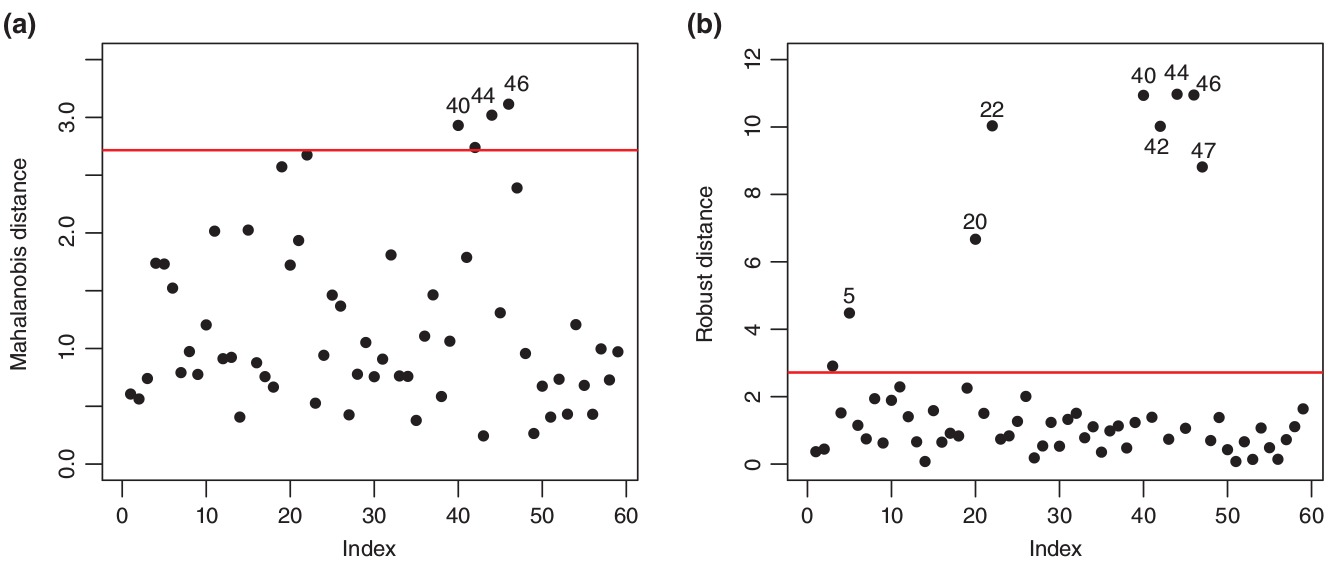
\includegraphics[width=11cm]{figures/mahalanobis_robust.png}
%      \caption{Mahalanobis Distance for non-robust and robust estimates.}
%      \label{fig:fig04}
% \end{figure}

% \begin{figure}[h!]
%      \centering
%      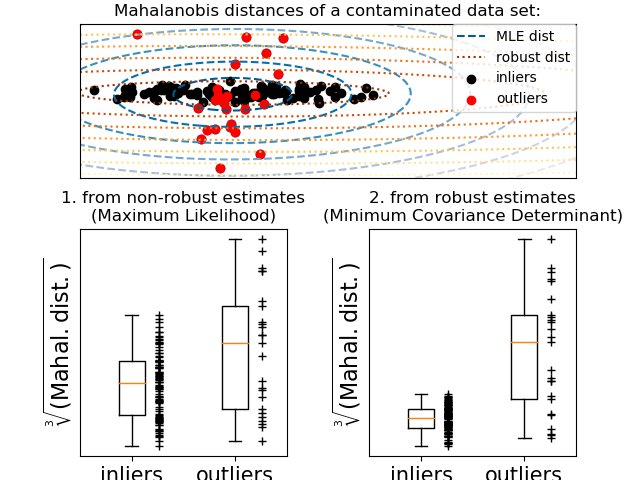
\includegraphics[width=8cm]{figures/mahalanobis_distances01.png}
%      \caption{Mahalanobis Distance for non-robust and robust estimates.}
%      \label{fig:fig05}
% \end{figure}

% The MCD estimator is one of the first affine equivariant and highly robust estimators of multivariate location and scatter.
		
% Affine equivariant means that when the data are translated or subjected to a linear transformation, the resulting location and scatter will transform accordingly \cite{rousseeuw1984mcd,rousseeuw1999fastmcd}.

% Its objective is to find $h$ observations (out of $n$) whose covariance matrix has the lowest determinant.

% The lowest determinant means the lowest distance generalized variance and high distance between the largest eigenvalue and the remaining [ref?].

% MCD depends on random sampling, therefore it is not deterministic.

% MCD has been applied in numerous fields (medicine, finance, image analysis, and chemistry) and been used to develop many robust multivariate techniques (such as Robust Principal Component Analysis (RPCA), factor analysis, and multiple regression).

% The classical MCD has rarely been applied because it is hard to compute, since it requires the evaluation of all $\binom{n}{h}$ subsets of size $h$. % binomial of n over p

% Its main use has started since the construction of the computationally efficient Fast-MCD algorithm \cite{rousseeuw1999fastmcd}.

% Fast-MCD is an iterative, approximate and resampling algorithm for the MCD.

% It starts by random initial subset of size $p+1$ and performs concentration steps (C-steps) yielding consecutive h-subsets with decreasing covariance matrix determinant.

% Only two C-steps are applied to each initial subset, and the 10 results with lowest determinant are kept.

% C-steps are carried out until convergence and the best solution is kept.

% Fast-MCD also is affine equivariant and not deterministic.
	
% \textbf{Theorem 1: C-Step.} 

% Consider a data set $\boldsymbol{X} \in \mathbb{R}^{n \times p}$ where $\boldsymbol{X} = \{\boldsymbol{x}_1,...,\boldsymbol{x}_n\}$ of $p$-variate observations. Let $\boldsymbol{h} \subset \{1,...,n\}$ with $|\boldsymbol{h}| = h$, where $\boldsymbol{h}$ is a subset of $h$ indexes from $n$ observations.

% Let the mean $\bar{\boldsymbol{x}} \in \mathbb{R}^{1 \times p}$ be

% \begin{equation}\label{eq:eq02}
% 	\bar{\boldsymbol{x}} = \displaystyle\frac{1}{h}\displaystyle\sum_{j\in \boldsymbol{h}} \boldsymbol{x}_j, 
% \end{equation}

% the covariance matrix $\boldsymbol{\hat{S}} \in \mathbb{R}^{p \times p}$ be

% \begin{equation}\label{eq:eq03}
% 	\boldsymbol{\hat{S}} = \displaystyle\frac{1}{h}\displaystyle\sum_{j\in \boldsymbol{h}} (\boldsymbol{x}_j - \bar{\boldsymbol{x}})(\boldsymbol{x}_j - \bar{\boldsymbol{x}})^\prime,
% \end{equation}

% and the relative distance be 	

% \begin{equation}\label{eq:eq04}
% 	\boldsymbol{d}(i) = \sqrt{(\boldsymbol{x}_i - \bar{\boldsymbol{x}}) \boldsymbol{\hat{S}}^{-1}(\boldsymbol{x}_i - \bar{\boldsymbol{x}})^\prime}, 
% \end{equation}

% for $i = 1,...,n$.

% Let $\boldsymbol{h}_1, \bar{\boldsymbol{x}}_1$ and $\boldsymbol{\hat{S}}_1$ and be the selected observations, the location and scatter of the initial subset, and $\boldsymbol{d}_1(i)$ be the initial distances for $i = 1,...,n$. 

% Now take $\boldsymbol{h}_2$ containing the indexes of lowest distances, such that $\{\boldsymbol{d}_1(i); i \in \boldsymbol{h}_2\} = \{(\boldsymbol{d}_1)_{1:n},...,(\boldsymbol{d}_1)_{h:n}\}$, where $(\boldsymbol{d}_1)_{1:n} \leq (\boldsymbol{d}_1)_{2:n} \leq ... \leq (\boldsymbol{d}_1)_{n:n}$ are the ordered distances, and compute $\boldsymbol{\bar{x}}_2$ and $\boldsymbol{\hat{S}}_2$ for $\boldsymbol{h}_2$.
	
% Then, $det(\boldsymbol{\hat{S}}_2) \leq det(\boldsymbol{\hat{S}}_1)$ with equality if and only if $\boldsymbol{\bar{x}}_2 = \boldsymbol{\bar{x}}_1$ and $\boldsymbol{\bar{S}}_2 = \boldsymbol{\hat{S}}_1$

% The proof is given by Rousseeuw and Driessen \cite{rousseeuw1999fastmcd}.
	
% \textbf{The C-step can be algorithmically described as follows:}
% \begin{algorithm}
% 	\label{alg:alg01}
% 	\scriptsize
% 	\SetAlgoLined
% 	\KwResult{$\boldsymbol{\bar{x}}_2$, $\boldsymbol{\hat{S}}_2$}
% 	Given the initial $h-$subset $\boldsymbol{h}_1$ of indexes or the pair $(\boldsymbol{\bar{x}}_1, \boldsymbol{\hat{S}}_1)$\;
% 	\While{$det(\boldsymbol{\hat{S}}_2) < det(\boldsymbol{\hat{S}}_1)$}{
% 		\If{$\boldsymbol{\bar{x}}_2$ and $\boldsymbol{\hat{S}}_2$ exist}{
% 			Put $\boldsymbol{\bar{x}}_1 = \boldsymbol{\bar{x}}_2$ and $\boldsymbol{\hat{S}}_1 = \boldsymbol{\hat{S}}_2$\;
% 		}
% 		Compute the distances $\boldsymbol{d}_1( i )$ for $i = 1,..., n$\;
% 		Sort $\boldsymbol{d}_1( i )$, which yields an index $\boldsymbol{d}_1(\pi(1)) \leq ... \leq \boldsymbol{d}_1(\pi(n))$\;
% 		Put $\boldsymbol{h}_2 = \{ \pi(1), \pi(2), ..., \pi(h)\}$\;
% 		Compute $\boldsymbol{\bar{x}}_2$ and $\boldsymbol{\hat{S}}_2$ for $\boldsymbol{h}_2$\;
% 		Compute $det(\boldsymbol{\hat{S}}_2)$ and $det(\boldsymbol{\hat{S}}_1)$\;			
% 	}
% 	\caption{C-Step}
% \end{algorithm}

% \textbf{Theorem 1} thus provides a partial idea for an algorithm: 

% \textit{Take many initial choices of $\boldsymbol{h}_1$ and apply C-steps to each until convergence (don't have determinant decreasing), and keep the result with lowest determinant}.

% \textbf{Initial subset can be algorithmically described as:}
% \begin{algorithm}
% 	\label{alg:alg02}
% 	\scriptsize
% 	\SetAlgoLined
% 	\KwResult{$\boldsymbol{h}_1$}
% 	Given a data set $\boldsymbol{X} \in \mathbb{R}^{n \times p}$ with $p$-variate observations\;
% 	Draw a random $(p + 1)$-subset $\boldsymbol{L}$\;
% 	Compute $\boldsymbol{\bar{x}}_1$ and $\boldsymbol{\hat{S}}_1$ of $\boldsymbol{L}$ and $det(\boldsymbol{\hat{S}}_1)$\;
% 	\If{$det(\boldsymbol{\hat{S}}_1) \leq 0$}{
% 		Add another random observation into $\boldsymbol{L}$\;
% 		Compute $\boldsymbol{\bar{x}}_1$ and $\boldsymbol{\hat{S}}_1$ of $\boldsymbol{L}$ and $det(\boldsymbol{\hat{S}}_1)$\;
% 	}
% 	Compute $\boldsymbol{d}_1^2(i) = (\boldsymbol{x}_i - \boldsymbol{\bar{x}}_1)^\prime \boldsymbol{\hat{S}}_1^{-1}(\boldsymbol{X}_i - \boldsymbol{\bar{x}}_0)$ for $i = 1, ..., n$\;
% 	Sort them into $\boldsymbol{d}_1(\pi(1)) \leq ... \leq \boldsymbol{d}_0(\pi(n))$\;
% 	Put $\boldsymbol{h}_1 = \{\pi(1), ..., \pi(h)\}$\;
% 	\caption{Constructing the initial subset}
% \end{algorithm}

% \begin{algorithm}
% 	\label{alg:alg03}
% 	\scriptsize
% 	\SetAlgoLined
% 	\KwResult{$\boldsymbol{\bar{x}}_2$, $\boldsymbol{\hat{S}}_2$}
% 	Given $\boldsymbol{X} \in \mathbb{R}^{n \times p}$, $h < n$, $p \geq 2$ and $n \leq 600$\;
% 	\For{500 times}{
% 		Construct initial $h$-subset $\boldsymbol{h}_1$ (Algorithm \ref{alg:alg02})\;
% 		Carry out two C-steps (Algorithm \ref{alg:alg01}) resulting $\boldsymbol{\bar{x}}_2$ and $\boldsymbol{\hat{S}}_2$\;
% 	}		
% 	Put $\boldsymbol{h}_1$ as the 10 lowest $det(\boldsymbol{\hat{S}_2})$ computed above\;
% 	\While{$det(\boldsymbol{\hat{S}}_2) < det(\boldsymbol{\hat{S}}_1)$}{
% 		Carry out C-steps (Algorithm \ref{alg:alg01})\;
% 	}
% 	\caption{Fast-MCD when $n \leq 600$}
% \end{algorithm}

% \begin{algorithm}
% 	\label{alg:alg04}
% 	\scriptsize
% 	\SetAlgoLined
% 	\KwResult{$\boldsymbol{\bar{x}}_2$, $\boldsymbol{\hat{S}}_2$}
% 	Given $\boldsymbol{X} \in \mathbb{R}^{n \times p}$, $h < n$, $p \geq 2$ and $n > 600$\;
% 	Construct up to 5 disjoint random subsets of size $n_{sub} = 300$\;
% 	\For{each subset, repeat 100 times}{
% 		Construct initial $\boldsymbol{h}_1$ of size $h_{sub} = [n_{sub}(h/n)]$\;
% 		Carry out two C-steps of $n_{sub}$ and $h_{sub}$\;
% 		Keep the 10 best $(\boldsymbol{\bar{x}}_{sub}, \boldsymbol{\hat{S}}_{sub})$\;
% 	}		
% 	Pool the subsets, yielding the merged set of $n_{merged} = 1500$\;
% 	\For{50 best $(\boldsymbol{\bar{x}}_{sub}, \boldsymbol{\hat{S}}_{sub})$}{
% 		Carry out two C-steps of $n_{merged}$ and $h_{merged} = [n_{merged}(h/n)]$\;
% 		Keep the 10 best $(\boldsymbol{\bar{x}}_{merged}, \boldsymbol{\hat{S}}_{merged})$\;
% 	}
% 	\For{the full data set and $m_{full}$ best results}{
% 		Take several C-steps, using $n$ and $h$\;
% 		Keep the best final result $(\boldsymbol{\bar{x}}_{full}, \boldsymbol{\hat{S}}_{full})$\;
% 	}
% 	\caption{Fast-MCD when $n > 600$}
% \end{algorithm}

% \cite{garcia2014empirical} proposed CTU-13 data set and argues that for evaluations of anomaly detection, none of the botnet families used in the training and crossvalidation data set should be used in the testing data set, considering that this ensures that the methods can generalize and detect new behaviors. However, hour proposal is semi-supervised and does not rely on training data with anomalies. Adopting the training and testing approach of \cite{garcia2014empirical}, some botnets malware wouldnt be evaluated, since in Garcia's proposal some botnets are present only for training. Therefore, we evaluate each scenario individually.

% \cite{wang2017botnet}
% A. Description of CTU-13 data set
% The CTU-13 is a data set of botnet traffic that was captured
% in the Czech Technical University [24]. It contains 13 scenarios
% with various botnet types. We consider scenarios 1, 2, 6, 8, and
% 9 of the data set.
% • Scenario 1 corresponds to an IRC-based botnet that sent spam for almost 6.5 hours.
% • Scenario 2 (2.5-hours) is from the same botnet.
% • Scenario 6 is from a botnet that scanned SMTP (Simple Mail Transfer Protocol) servers for 2 hours and connected to several RDP (Remote Desktop Protocol) services. Dif-erent with Scenarios 1 and 2, this botnet neither sent spam nor did it attack. It’s C\&C server used a proprietary protocol.
% • Scenario 8 is from a botnet that contacted a lot of Chinese C\&C hosts and received large amounts of encrypted data. The botnet also cracked the passwords of machines during the 19-hour attack.
% • Scenario 9 corresponds to a case where 10 local hosts were infected by a spamming botnet. More than 600 spams were sent over 5 hours.